\input{arbeit-vorlage-praeambel.tex} % Importiere die Einstellungen aus der Präambel
% hier beginnt der eigentliche Inhalt
\begin{document}
\pagenumbering{Roman} % Seitenummerierung mit großen römischen Zahlen 
\pagestyle{empty} % keine Kopf- oder Fußzeilen auf den ersten Seiten

% Titelseite
\clearscrheadings\clearscrplain
\begin{center}
\begin{Huge}
Universität Bremen\\
\vspace{3mm}
\end{Huge}
{\Large Fachbereich 3}\\

\vspace{20mm}
\begin{Large}
Robotergestütztes Kalibrierungssystem für Sensoren\\
\end{Large}
\vspace{8mm}
Bachelorarbeit\\
\vspace{0.4cm}
\vspace{2 cm}
Benny Prange \\
Matrikel-Nummer 2597237\\
10.08.2017\\
\vspace{8cm}
\begin{tabular}{rl}
{\bfseries Betreuer} & Alexis Maldonado\\
{\bfseries Erstprüfer}&Prof. Dr. Michael Beetz\\
{\bfseries Zweitprüfer}&Dr. Karsten Sohr\\
\end{tabular}

\end{center}
\clearpage


\pagestyle{useheadings} % normale Kopf- und Fußzeilen für den Rest

\tableofcontents % erstelle hier das Inhaltsverzeichnis
\listoffigures % erstelle hier das Abbildungsverzeichnis
\listoftables % erstelle hier das Tabellenverzeichnis
\clearpage

\pagenumbering{arabic} % ab jetzt die normale arabische Nummerierung

\chapter{Einleitung}

In der Robotik werden bildgebende Sensoren benutzt, um Informationen über das Umfeld des Roboters zu erhalten. Diese Informationen können genutzt werden, um Hindernisse zu erkennen, die der Roboter meiden soll oder es werden Gegenstände gesucht, die der Roboter greifen und mit ihnen interagieren soll. Es gibt verschiedene Arten von bildgebenden Sensoren, wie z.B. Kameras, die ein zweidimensionales Bild erzeugen und Kameras, die zusätzlich zu dem zweidimensionalen Bild auch Tiefeninformationen erkennen. Andere Sensoren, die ein räumliches Abbild ohne Farbinformationen erstellen, sind z.B. Lidar-, Ultraschall- und Radarsensoren.

Bei all diesen Sensoren ist es wichtig, dass diese korrekt kalibriert sind, damit die gemessenen Daten der Realität möglichst nahe kommen. Stimmen die Messdaten nicht mit der Realität überein, stößt der Greifarm ein Objekt möglicherweise um, anstatt es zu greifen.

Kamerasensoren, die nach dem Lochkameraprinzip arbeiten, werden durch die Kameramatrix definiert. Sie enthält Angaben über den internen Aufbau der Kamera, wie Bildsensorgröße und Brennweite, sowie die Position der Kamera in Relation zu der realen Umgebung. Dadurch lassen sich aus einem aufgenommenen Bild Informationen über die dreidimensionale Welt berechnen. 

Das Ziel der Kalibirierung einer Kamera ist es, eine Kameramatrix zu berechnen, die eine möglichst exakte Relation von Kamerabildern zu der realen Umgebung ermöglicht. Diese Kameramatrix kann mithilfe von Kalibriermustern erstellt werden. Dazu werden mehrere Fotos aufgenommen, auf denen das Muster in verschiedenen Entfernungen und Orientierungen zu sehen ist. Schließlich lässt sich aus diesen Daten die Kameramatrix berechnen.

Dieser Vorgang ist sehr zeitaufwändig. Zum einen müssen viele Bilder gemacht werden, um eine möglichst präzise Kalibrierung zu erhalten. Daher werden bis zu 50 Bilder aufgenommen. Zum anderen empfiehlt es sich, Kamera und Kalibiriermuster jeweils auf einem Stativ zu befestigen, um scharfe Bilder zu erzeugen. Damit ist gewährleistet, dass die Erkennung des Kalibriermusters nicht von unscharfen Bildern gestört wird, allerdings wird der Vorgang durch das Verstellen der Stative auch weiter verlängert.

Um die Kalibrierung zu vereinfachen, soll daher ein Roboterarm das Bewegen des Kalibriermusters übernehmen und der ganze Ablauf mit dem Erstellen der Bilder und dem Berechnen der Parameter durch ein Programm gesteuert werden. Der Benutzer platziert die Kamera auf einem Stativ vor dem Roboterarm, an dem das Kalibiriermuster befestigt ist. Anschließend startet er das Programm, welches den Arm an verschiedene Positionen bewegt, sodass die Kamera das Muster aus mehreren Entfernungen und Orientierungen aufnehmen kann. Zum Schluss berechnet das Programm die benötigten Parameter und der Benutzer kann die Kamera mit diesen Parametern einsetzen.
\chapter{Grundlagen}
\label{chap:grundlagen}

Wie bereits in der Einleitung erwähnt sind Kameras ein wichtiger Sensor in der Robotik, undem sie dem Roboter helfen, die Umgebung wahrzunehmen. Abhängig von dem Einsatzgebiet ist ein genaues Abbild der Umgebung außerordentlich wichtig für die Erfüllung der Aufgabe. Dies ist der Fall wenn zum Beispiel der Roboter über das Kamerabild einen Gegenstand lokalisieren muss, um ihn anschließend zu greifen, oder er muss in dem Kamerabild Hindernisse erkennen, um einen Weg zum Ziel zu planen.

Der relativ günstige Preis von Lochkameras gegenüber anderen bildgebenden Sensoren hat dazu beigetragen, dass Kameras ein viel genutzter Sensor sind. Da sich aber gezeigt hat, dass die Toleranzen bei der Produktion und der Aufbau der Kameras an sich zu Verzerrungen im Bild führen, wurden Modelle entwickelt, um diese Verzerrungen herauszurechnen und das Bild zu korrigieren. Ein häufig genutztes Modell wird im folgenden beschrieben.

\section{Kameramodell} % (fold)
\label{sec:kameramodell}
In \cite{Zhang} wird ein gängiges Kameramodell beschrieben, welches nun kurz erklärt wird.

Die Beziehung zwischen einem Punkt in einem zweidimensionalen Bild und einem Punkt in der dreidimensionalen Welt wird durch \autoref{projection} beschrieben:

\begin{equation}
\begin{bmatrix}
 	u \\
 	v \\
 	1
\end{bmatrix} = K 
\begin{bmatrix}
   	R & T
\end{bmatrix} 
\begin{bmatrix}
   	x \\
   	y \\
   	z \\
   	1
\end{bmatrix} \label{projection}
\end{equation}

mit 

\begin{equation}
  K = 
  \begin{bmatrix}
  	f_x & 0 & c_x \\
  	0 & f_y & c_y \\
  	0 & 0 & 0
  \end{bmatrix}
\end{equation}

$K$ enthält die intrinsischen Parameter der Kamera, die auf Grund der Fertigungstoleranzen für jede Kamera unterschiedlich sind. $f$ definiert die Brennweite der Kamera. Da die Pixel nicht immer quadratisch sind, wird dieser Wert für die x und y-Achse angegeben. $c_x$ und $c_y$ beschreiben das optische Zentrum des Bildes, welches ebenfalls nicht immer genau im Mittelpunktes des Bildes liegt.

$R$ und $T$ definieren die extrinischen Parameter. $R$ ist eine Rotationsmatrix, die die Rotation zwischen dem Kamera- und Weltkoordinatensystem beschreibt, $T$ ist ein Vektor der die Transformation zwischen Kamera- und Weltkoordinatensystem beschreibt.

\section{Verzeichnung} % (fold)
\label{sec:verzeichnung}
Mit dem Kameramodell kann nun eine Beziehung zwischen einem Punkt im Bild und dem Punkt in der Welt hergestellt werden. Kameras bilden das Bild jedoch nicht immer korrekt ab. Häufig sieht man in Bildern den Effekt, dass gerade Linien in der Welt, wie z.B. Häuserkanten nicht gerade im Bild aufgenommen werden, sondern das diese im Bild gebogen werden. Diesen Effekt nennt man Verzeichnung.

Man kann zwischen zwei verschiedenen Arten der Verzeichnung sprechen. Die Verzeichnung, die gerade Linien gekrümmt darstellt, heißt radiale Verzeichnung. Um diese Verzeichnung herauszurechnen werden die drei Faktoren $k_1, k_2, k_3$ benötigt. Sind diese gegeben, lässt sich die Verzeichnung korrigieren. $r$ ist der Abstand vom Bildmittelpunkt zum Punkt, der korrigiert werden soll. $x', y'$ sind die falsch abgebildeten Punkte, $x,y$ sind die korrigierten Punkte.

\begin{equation}
	x = x'(1 + k_1 r^2 + k_2 r^4 + k_3 r^6)
\end{equation}
\begin{equation}
	y = y'(1 + k_1 r^2 + k_2 r^4 + k_3 r^6)
\end{equation}

Zusätzlich zu der radialen Verzeichnung gibt es tangentiale Verzeichnung. Diese tritt auf, wenn die Kameralinse nicht parallel zum Sensor eingebaut ist. Diese Verzeichnung führt dazu, dass Linien, die im idealen Bild parallel verlaufen, nun einen gemeinsamen Fluchtpunkt besitzen. Um diese Verzeichnung zu korrigieren, werden die Faktoren $p_1, p_2$ benötigt.

\begin{equation}
	x = x' + (2 p_1 xy + p_2 (r^2 + 2 x^2))
\end{equation}
\begin{equation}
	y = y' + (p_1(r^2 + 2 y^2) + 2p_2 xy)
\end{equation}
%!TEX root = ../bachelorthesis.tex
\chapter{Architektur}
\label{chap:architektur}
Für dieses Projekt wurden mehrere Softwareprogramme integriert, teilweise wurden eigene Programme geschrieben. In den folgenden Abschnitten wird ein Gesamtüberblick gegeben und die einzelnen Programme werden hinsichtlich ihrer Aufgaben detailliert beschrieben.

\section{Gesamtübersicht} % (fold)
\label{sec:gesamtübersicht}
In \autoref{img:overview} ist die Architektur graphisch dargestellt. Jeder Knoten stellt dabei eine ROS-Node dar, also ein einzelnes Programm. Knoten, die blau eingefärbt sind, stehen für Programme, die von anderen Benutzern programmiert wurden und gegebenenfalls zu diesem Einsatzzweck angepasst wurden. Programme, die im Rahmen dieser Bachelorarbeit programmiert wurden, sind grün eingefärbt.
\begin{figure}[!hbt]
	\centering
	\vspace{1ex}
	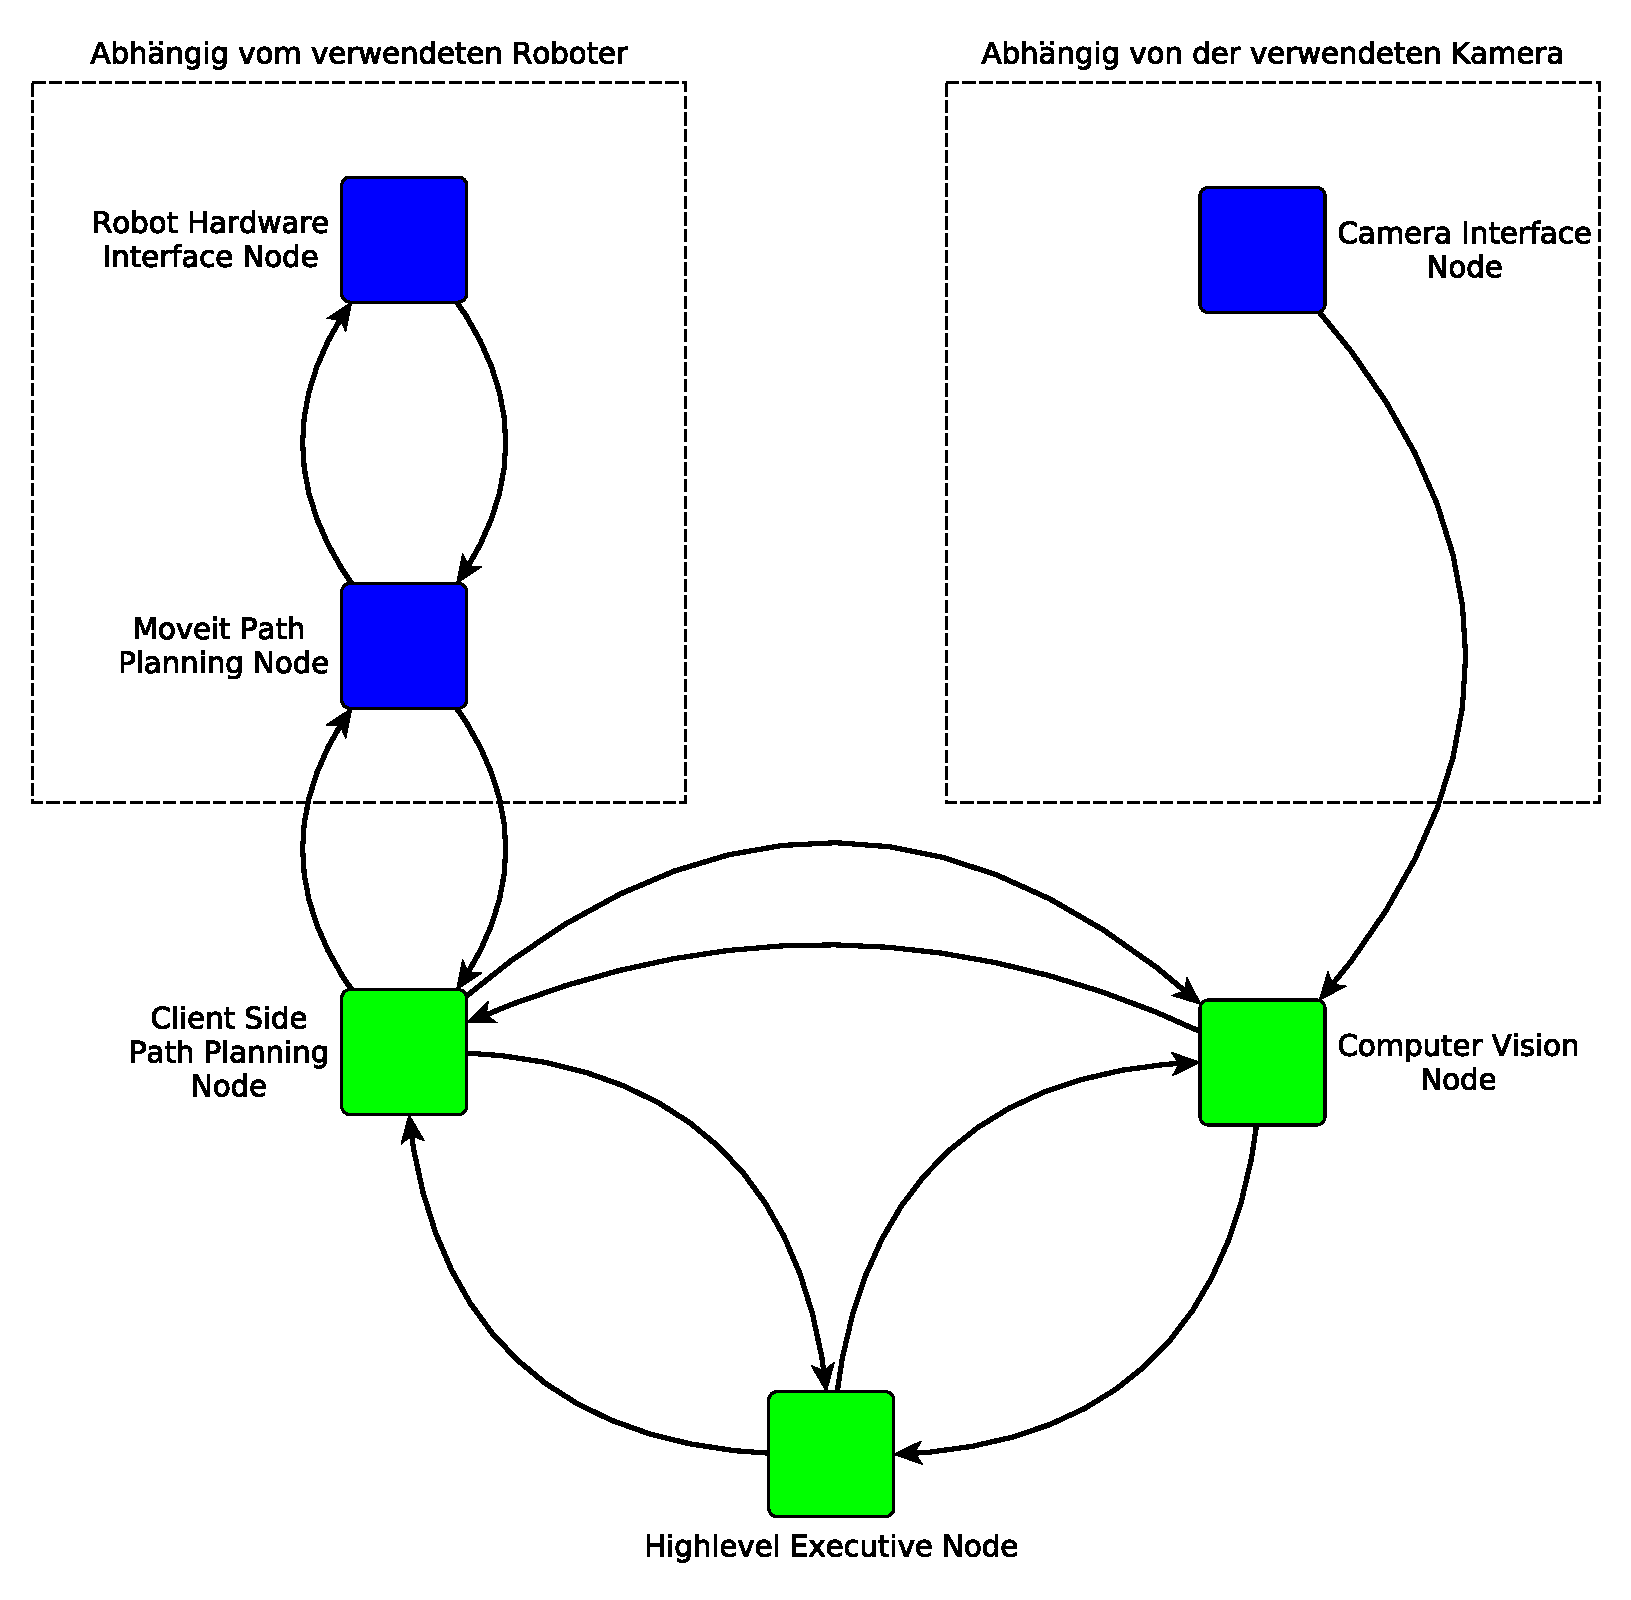
\includegraphics[scale=0.6]{../images/overview}
	\caption[Übersicht über die Architektur. Die Pfeile verdeutlichen die Kommunikation zwischen den Knoten.]{\label{img:overview} Übersicht über die Architektur}
	\vspace{1ex}
\end{figure}
\todo{Übersetzung von Architekturnamen zu tatsächlichen Klassennamen fehlt.}
Die Robot Hardware Interface Node stellt eine Schnittstelle bereit, damit ROS-Pakete wie MoveIt! den Roboter steuern können.

Die Moveit Path Planning Node startet MoveIt! und die dazugehörigen Programme, um MoveIt! zum Planen und Ausführen von Bewegungen nutzen zu können.

Die Camera Interface Node veröffentlicht das Kamerabild über einen ROS Topic.

Die Client Side Path Planning Node stellt eine weitere Abstraktionsschicht zur Bewegung des Arms zur Verfügung. Sie bereitet die Positionsziele für MoveIt! auf und startet die Auswertung von Bildern.

Die Computer Vision Node wertet die empfangenen Bilder der Kamera aus.

Die Highlevel Executive Node steuert den gesamten Ablauf.

\section{Robot Hardware Interface Node} % (fold)
\label{sec:ur_modern_driver}
Für diese Node wird das Paket \texttt{ur\_modern\_driver} verwendet, siehe \cite{ur_modern_driver}. Sie ist die Schnittstelle zwischen dem Roboterarm UR5 und dem ROS Framework. Da dieses Paket nicht für die in diesem Projekt benutzte Version von ROS entwickelt wurde, wurden einige wenige Anpassungen am Sourcecode vorgenommen, um das es in diesem Projekt benutzen zu können.

\section{Moveit Path Planning Node} % (fold)
\label{sec:universal_robot}
Auch für diese Node wird ein öffentlich verfügbares Paket genommen: \texttt{universal\_robot}, siehe \cite{universal_robot}. In dieser Node ist MoveIt! integriert, welches zum Bewegen des Roboterarms benutzt wird. Siehe \autoref{ssub:moveit} für weitere Details über MoveIt!.

\section{Camera Interface Node} % (fold)
\label{sec:libuvc_camera}
Auch diese Node ist als Paket \texttt{libuvc\_camera} in ROS verfügbar. Sie dient dazu, das Bild der angeschlossenen Webcam über ROS verfügbar zu machen. In dem Script, mit dem diese Node gestartet wird, lassen sich verschiedene Parameter einstellen. In diesem Fall wurde mittels der Vendor-ID und Product-ID die zu benutzende Kamera definiert, die Auflösung wurde auf Full-HD gesetzt und der Fokus wurde so eingestellt, dass der Bereich, in dem sich das Kalibrierungsmuster befinden wird, scharf zu sehen ist.

\section{Client Side Path Planning Node} % (fold)
\label{sec:movearmserver}
Dieses Programm wurde im Rahmen dieser Bachelorarbeit selbst entwickelt. Es dient dazu, der Highlevel Executive Node eine weitere Abstraktionsschicht zum Bewegen des Arms zu bieten.

Dazu wurde ein Actionserver erstellt, der die Position des Kalibrierungsmusters als Auftrag erhält. Zusätzlich kann als weiterer Parameter für den Auftrag die Neigung des Musters angegeben werden. Das Programm berechnet dann für die gewünschte Position zunächst die Orientierung für den Roboterendpunkt, damit das Muster senkrecht zur Kamera steht. Anschließend wird zu der berechneten Orientierung die gewünschte Neigung hinzugefügt. Die so errechnete Position und Orientierung wird dann an MoveIt! übergeben. Abhängig davon, ob MoveIt! den Arm erfolgreich bewegen konnte, informiert diese Node den Highlevel Executive Controller, ob der Auftrag erfolgreich ausgeführt wurde.

\section{Computer Vision Node} % (fold)
\label{sec:caltab_detector_node}
Auch dieses Programm wurde selbst entwickelt. Es benutzt die Bibliothek von HALCON, um in den Bildern, die es von der Kamera empfängt, nach dem Kalibrierungsmuster zu suchen und die Kalibrierung durchzuführen.

Diese Node bietet zwei Actionserver an. Der erste Actionserver erwartet einen Auftrag, um in den aktuellen Bildern nach dem Kalibrierungsmuster zu suchen. Dazu wird ein Parameter übergeben, der angibt, wie viele Bilder ausgewertet werden sollen. Die Algorithmen von HALCON finden nicht immer im ersten Versuch das Muster, daher lässt sich die Anzahl der Bilder mit Hilfe dieses Parameters definieren. Die Node meldet dem Highlevel Executive Controller zurück, ob nach der angegeben Anzahl der Bilder das Muster gefunden wurde oder nicht.

Der zweite Actionserver nimmt den Auftrag zur Durchführung der Kalibrierung an. Dazu werden die Bilder, in denen das Muster zu sehen war, ausgewertet. Danach werden die errechneten intrinsischen Parameter, die Verzeichnungsparameter sowie der ermittelte durchschnittliche Fehler an den Highlevel Executive Controller zurückgegeben.

\section{Highlevel Executive Controller} % (fold)
\label{sec:calibrationcontroller}
Diese letzte Node wurde ebenfalls selbst entwickelt. Sie dient dazu, den gesamten Ablauf der Kalibrierung zu steuern, indem sie die Actionserver mit Aufgaben versorgt. Zunächst übergibt der Benutzer dem Programm die Position der Kamera in Relation zur Basis des Roboterarms und die initialen intrinsischen Parameter. Dann wird aus diesen Werten das Sichtfeld der Kamera bestimmt. Mit diesem Sichtfeld werden danach die verschiedenen Distanzen zur Kamera berechnet und anschließend die Positionen für das Kalibrierungsmuster, damit dieses das ganze Sichtfeld der Kamera abdeckt.

Diese Positionen werden nacheinander an den MoveArmServer übergeben. Für jede Position wird das Muster nach oben, unten, rechts und links geneigt. Hat der Actionserver den Auftrag erfolgreich ausgeführt, wird der Computer Vision Node der Auftrag übergeben, in dem Kamerabild nach dem Muster zu suchen. Ist dieser Auftrag abgeschlossen, wird die nächste Position angesteuert.

Wurden alle Positionen abgearbeitet, wird zum Schluss der Auftrag zur Kalibrierung durchgeführt. Die dadurch erhaltenen Parameter werden dem Benutzer angezeigt und das Programm hat seine Durchführung beendet.
%!TEX root = ../bachelorthesis.tex
\chapter{Implementierung}
\label{chap:implementierung}
Nachdem der grundsätzliche Aufbau und Ablauf der Kommunikation des Gesamtprogramms beschrieben wurde, werden nun die Details der einzelnen Module dargestellt.

\section{Moveit Path Planning Node} % (fold)
\label{sec:universal_robot_impl}

An diesem Programm wurden einige Anpassungen vorgenommen. Zum einen wurde die in MoveIt! benutzte Bibliothek zur Lösung der inversen Kinematik KDL durch TRAC\_IK ausgetauscht. Diese Bibliothek wird dazu verwendet, für eine gewünschte Position und Orientierung des Roboterarms die dazu erforderlichen Winkel der Gelenke zu berechnen. Während der Versuche war es teilweise zu beobachten, dass MoveIt! keinen oder nur einen viel zu komplizierten Weg von der Start- zur Zielkonfiguration gefunden hat. Dieses Problem konnte teilweise durch diesen Austausch mit TRAC\_IK behoben werden.

Zusätzlich wurde das URDF in diesem Paket angepasst. Das URDF enthält die geometrischen Informationen über den Roboterarm, wie z.B. die Länge und Form der einzelnen Glieder und die Position der Werkzeugaufnahme des Arms. Wird dem Arm eine Zielposition und Orientierung übergeben, so gilt diese normalerweise für diese Werkzeugaufnahme. Für die Bachelorarbeit wurde jedoch das Kalibrierungsmuster an diese Stelle montiert. Das Muster wurde nicht mittig an der Werkzeugaufnahme angebracht, sondern steht seitlich ab. Daher wurde im URDF der Endpunkt des Arms von der Werkzeugaufnahme auf den Mittelpunkt des Kalibrierungsmusters versetzt. Das führt dazu, dass sich nun nicht mehr die Werkzeugaufnahme des Arms an der Zielposition befindet, sondern der Mittelpunkt des Kalibrierungsmusters.
\todo{Foto vom Caltab am Endeffector}

\section{Client Side Path Planning Node} % (fold)
\label{sec:movearmserver_impl}
Diese Node wurde in der Programmiersprache Python entwickelt und hat den Namen \texttt{MovementHandler.py}. Sie hat den Auftrag, die Bewegung des Arms zu koordinieren und dazu mit MoveIt! zu kommunizieren.

Das Programm erhält beim Start die Position der Kamera in Relation zur Basis des Arms. Außerdem wird ein Actionserver gestartet, der auf Aufgaben vom Typ \texttt{move\_arm} wartet. Zusätzlich wird der Kommunikationskanal zu MoveIt! gestartet.

Die Aufgabe \texttt{move\_arm} ermöglicht es einem Actionclient, den Roboterarm zu einer von ihm gewählten Position zu bewegen. Zusätzlich kann er die horizontale und vertikale Neigung des Musters bestimmen.

Erhält das Programm eine Aufgabe, so wird zunächst für die gewünschte Position die Orientierung des Arms berechnet. Dazu wird zunächst angenommen, dass das Kalibrierungsmuster orthogonal zur Kamera stehen soll. Jede Position lässt sich mit den drei Variablen $x, y, z$ definieren. Dadurch lässt sich jede Position auch als Ortsvektor darstellen:
\begin{equation}
	\vec{p} = 
	\begin{pmatrix}
		x\\
		y\\
		z
	\end{pmatrix}
\end{equation}

Um nun die Orientierung zu errechnen, subtrahiert man zunächst den Vektor für die Position der Kamera vom Vektor für die Position des Roboterarms. Der daraus resultierende Vektor $\vec{p}_{diff}$ beschreibt die geometrische Transformation vom Arm zur Kamera. 
\begin{equation}\label{eq:diff}
	\vec{p}_{Diff} = \vec{p}_{Roboter} - \vec{p}_{Kamera}
\end{equation}
Mit diesem Vektor lässt sich nun der Gierwinkel $\alpha$ und Neigungswinkel $\beta$ bestimmen, damit das Muster orthogonal zur Kamera steht:
\begin{equation}\label{eq:pitch}
	\alpha = \arctantwo(y_{diff}, x_{diff})
\end{equation}
\begin{equation}\label{eq:yaw}
	\beta = -\arcsin(x_{diff})
\end{equation}

Mit diesen Winkeln würde nun das Muster orthogonal zur Kamera zeigen. Wurden in der Aufgabe zusätzliche Neigungen angegeben, werden diese nun zu diesen Winkeln addiert.

Schließlich muss noch der Rollwinkel $\gamma$ bestimmt werden. In diesem Anwendungsfall soll das Kalibrierungsmuster immer nach außen zeigen und parallel zum Boden stehen, damit die Reichweite des Roboters erhöht wird. Dazu wird die folgende Gleichung gelöst:
\begin{equation}
	\gamma = \arctantwo(y_{Roboter}, x_{Roboter}) - \arctantwo(y_{Kamera}, x_{Kamera})
\end{equation}
Ist $\gamma > 0$, so befindet sich das Muster von der Kamera aus gesehen in der rechten Hälfte des Bildes. Damit das Muster nach außen zeigt, muss der Rollwinkel 0$^\circ$ betragen. Ist $\gamma < 0$, befindet sich das Muster in der linken Hälfte und der Rollwinkel wird auf 180$^\circ$ gesetzt.

Wurde die Orientierung berechnet, muss für die Position und Orientierung ein Plan generiert werden, mit dem sich der Arm aus der Startposition zur Zielposition bewegt, ohne dass er mit sich selbst oder der Umgebung kollidiert. Diese Aufgabe übernimmt MoveIt!. Aufgrund des eingesetzten Algorithmus in MoveIt! können für gleiche Start- und Zielpositionen unterschiedliche Pläne erstellt werden, teilweise kann MoveIt! auch keinen Plan finden. Daher werden für jede Aufgabe, die der Actionserver erhält, fünf Pläne von MoveIt! erzeugt. Wenn die gewünschte Position nicht erreichbar ist oder Teile des Roboters oder das Kalibrierungsmuster mit sich selber oder der Umgebung kollidieren würden, sind alle fünf Pläne leer. In diesem Fall wird die Aufgabe abgebrochen und dem Actionclient eine negative Rückmeldung zurückgegeben. Ansonsten wird der Plan ausgewählt, der die geringste Anzahl an Zwischenpositionen enthält, und an MoveIt! zur Ausführung übermittelt. Hat MoveIt! die erfolgreiche Ausführung bestätigt, wird dem Actionclient die Aufgabe positiv bestätigt.

\section{Computer Vision Node} % (fold)
\label{sec:caltab_detector_node_impl}
Diese Node wurde in der Programmiersprache C++ programmiert und liegt im Paket \texttt{caltab\_detector} mit dem Dateinamen \texttt{caltab\_detector\_node.cpp}. Sie dient dazu, die von der Kamera übermittelten Bilder auszuwerten und zur Kalibrierung vorzuhalten.

Vor dem Start muss der Benutzer über die Datei \texttt{caltab\_detector/config/parameters.yaml} einige Parameter konfigurieren. Diese sind in \autoref{tab:caltab_detector} aufgeführt.

\begin{table}
\begin{tabularx}{\textwidth}{|l|X|}
	\hline
	Parametername & Beschreibung \\\hline
	focal\_length & Brennweite in Metern \\\hline
	sensor\_size x & Größe des Sensors entlang der x-Achse in Metern \\\hline
	sensor\_size y & Größe des Sensors entlang der y-Achse in Metern \\\hline
	resolution x & Anzahl der Pixel des Bildes entlang der x-Achse \\\hline
	resolution y & Anzahl der Pixel des Bildes entlang der y-Achse \\\hline
	image\_topic & Der Name des Topics, auf dem die Bilder von der Kamera veröffentlicht werden \\\hline
	description\_file & Der Pfad zu der Datei, die die Beschreibung für das Kalibrierungsmuster enthält \\\hline
\end{tabularx}
\caption{Beschreibung der Parameter für die Computer Vision Node}
\label{tab:caltab_detector}
\end{table}

Über das angegebene Topic erhält das Programm die Bilder der Webcam. Zusätzlich stellt das Programm zwei Actionserver zur Verfügung. Der Actionserver mit dem Namen \texttt{find\_calibration\_object} hat die Aufgabe, in dem aktuellen Bild der Webcam nach dem Kalibrierungsmuster zu suchen. Der Actionclient kann für jeden Auftrag angeben, in wie vielen aufeinanderfolgenden Bildern der Server nach dem Muster suchen soll, da dieses nicht immer im ersten Versuch gefunden wird. Hat der Server das Muster innerhalb der erlaubten Anzahl von Bildern gefunden, erhält der Client eine positive Rückmeldung, ansonsten eine negative.

Der zweite Actionserver \texttt{Calibrate} führt die Kalibrierung durch und errechnet aus allen Bildern, in denen das Muster zu sehen war, die intrinsischen Parameter, die Verzeichnungsparameter und den mittleren Fehler. Zusätzlich werden diese Bilder auf der Festplatte abgespeichert. Für jedes Bild wird außerdem eine Kopie angefertigt, in der eine Simulation des Musters über das im Bild zu sehende Muster gelegt wird. Dadurch kann zusätzlich visuell die Qualität der Kalibrierung überprüft werden.

Beim Start der Node kann der Benutzer ein Verzeichnis angeben, in dem die Bilder gespeichert werden sollen. Andernfalls wird in dem aktuellen Verzeichnis ein Unterordner erstellt. Außerdem wird die Datei gelesen, in der die initialen intrinsischen Parameter für die eingesetzte Kamera hinterlegt sind. Ebenfalls wird die Datei gelesen, in der die Dimensionen und Eigenschaften des benutzten Kalibrierungsmusters definiert sind. Anschließend verbindet sich das Programm mit dem Topic der Kamera, um die Bilder zu empfangen.

Jedes Mal, wenn das Programm ein aktuelles Bild von der Kamera erhält, wird die Methode \texttt{subscriberCallback} aufgerufen. Die Methode überprüft zunächst, ob auf Grund eines laufenden Auftrags für den find\_calibration\_object Actionserver noch Bilder überprüft werden sollen. Ist dies nicht der Fall, wird die Methode direkt beendet und das Programm wartet weiter auf eingehende Aufträge oder neue Bilder. 

Wenn jedoch ein Auftrag aktiv ist und das aktuelle Bild ausgewertet werden soll, wird die Methode weiter abgearbeitet. Das empfangene Bild ist vom Typ \texttt{sensor\_msgs::Image}. Um es aber mit HALCON benutzen zu können, muss es zu dem Typ \texttt{HObject} umgewandelt werden. Dazu wird das Bild in einem Zwischenschritt mit Hilfe der Methode \texttt{toCvCopy} aus dem Paket \texttt{cv\_bridge} in ein Objekt vom Typ \texttt{cv::Mat} konvertiert. Dadurch kann man nun relativ einfach auf den Wert für jedes einzelne Pixel zugreifen. Anschließend wird Pixel für Pixel über das gesamte Bild iteriert und die Werte der Pixel werden in einem \texttt{unsigned char*} gespeichert. Die HALCON-Methode \texttt{GenImage1} liest dann die Werte aus dem \texttt{unsigned char*} und erstellt das \texttt{HObject}.

Für jedes auszuwertende Bild wird ein fortlaufender Index erstellt, der im weiteren Verlauf benötigt wird. Es wird nun die HALCON-Methode \texttt{FindCalibObject} aufgerufen. Diese sucht in dem eben erstellten Bild nach dem Kalibrierungsmuster. Wird das Muster nicht erkannt, wirft diese Methode eine Exception. Diese wird im weiteren Verlauf der \texttt{subscriberCallback}-Methode gefangen und in der Konsole wird die Fehlermeldung von HALCON ausgegeben. Kann HALCON das Muster erkennen, wird es intern unter dem Index abgespeichert und zusätzlich in dem vom Benutzer angegeben Ordner gespeichert. In einer von diesem Programm verwalteten Liste wird zusätzlich der Index dieses Bildes abgespeichert. Der boolesche Wert caltabFound wird auf wahr gesetzt und die Anzahl der noch auszuwertenden Bilder für den aktuellen Auftrag auf null. 

Erhält der find\_calibration\_object Actionserver einen neuen Auftrag, wird die Methode \texttt{find\_calibration\_objectAction} aufgerufen. Zunächst wird der boolesche Wert auf falsch und die Anzahl der auszuwertenden Bilder auf den Wert gesetzt, der im Auftrag vom Client angegeben wurde. Dann wartet die Methode so lange, bis entweder die angegebene Anzahl an Bildern ausgewertet wurde oder vorher ein Kalibrierungsmuster gefunden wurde. Ist der boolesche Wert caltabFound wahr, wird dem Client eine positive Rückmeldung gegeben, sonst eine negative.

Wenn der Calibrate Actionserver einen Auftrag erhält, wird die Kalibrierung durchgeführt. Dazu wird zunächst die HALCON-Methode \texttt{CalibrateCameras} aufgerufen. Diese berechnet intern die neuen intrinsischen Parameter und die Parameter für die Verzeichnung. Außerdem wird der mittlere Fehler zurückgegeben. Um nun die neuen Parameter zu erhalten, wird die HALCON-Methode \texttt{GetCalibData} aufgerufen. Die so erhaltenen Werte werden zunächst in Werte vom Typ \texttt{double} umgewandelt. Dann werden dem Client diese Werte, der Fehler und die Anzahl der zur Kalibrierung benutzten Bilder zurückgegeben.

Anschließend wird nacheinander jedes abgespeicherte Bild mit Hilfe der Liste, die alle Indizes enthält, noch einmal mit HALCON eingelesen. Zunächst wird für das Bild die Position und Orientierung des Kalibrierungsmuster von HALCON ausgelesen, wie es von HALCON erkannt wurde. Dann werden diese Informationen mit den neuen Kameraparametern korrigiert. Schließlich wird das so korrigierte Kalibrierungsmuster über das eingelesene Bild gelegt und das Bild so auf dem Dateisystem abgespeichert. Siehe dazu \autoref{img:example_caltab} und \autoref{img:example_caltab_added}.
\begin{figure}
\centering
\includegraphics[width=\textwidth]{images/example_caltab}
\caption{Das Originalbild.}\label{img:example_caltab}
\end{figure}
\begin{figure}
\centering
\includegraphics[width=\textwidth]{images/example_caltab_added}
\caption{Das Bild mit dem eingezeichneten Kalibrierungsmuster. Man beachte die feinen Linien, die um das schwarze Rechteck und in die Kreise eingefügt wurden.}\label{img:example_caltab_added}
\end{figure}

\section{MovementController} % (fold)
\label{sec:movementcontroller_impl}
Die Klasse MovementController wurde wieder in Python entwickelt. Sie agiert als Actionclient für den move\_arm Actionserver und den find\_calibration\_object Actionserver und koordiniert die Bewegung des Arms zu den verschiedenen Positionen und die anschließende Suche nach dem Kalibrierungsmuster im Bild. Sie wird vom High Level Executive gestartet.

Beim Start der Klasse über den \texttt{CalibrationController} kann ihr als Argument durch den Benutzer eine Verzögerung in Sekunden übergeben werden. Dies hat den Hintergrund, dass einige Kamerasensoren eine nicht unerhebliche Verzögerung zwischen der Bildaufnahme und dem Veröffentlichen über einen Topic aufweisen. Bei einer zu geringen Verzögerung zwischen dem Erreichen der Position und der Auswertung der Bilder kann der Arm auf den Bildern noch in Bewegung sein. Dadurch wird das Muster entweder an der falschen Stelle ausgewertet oder es ist so unscharf abgebildet, dass es nicht erkannt werden kann.

Die Klasse führt nach ihrer Initialisierung nichts weiter aus, sondern stellt dem \texttt{High Level Executive} die Methode \texttt{execute\_different\_orientations} zur Verfügung. Dieser Methode muss eine Position übergeben werden, an die das Kalibrierungsmuster bewegt werden soll. Für diese Position wird dann zunächst ein Bild ohne zusätzliche Neigung gemacht. Anschließend wird das Bild in 10$^\circ$-Schritten nach oben, unten, links und rechts geneigt, wobei für jede Orientierung wieder ein Bild aufgenommen wird. Dazu ruft der \texttt{MovementController} die Methode \texttt{take\_picture\_with\_orientation} auf. Dieser Methode wird ebenfalls die Position übergeben und zusätzlich die gewünschte horizontale und vertikale Neigung. Zunächst wird also diese Methode ohne zusätzliche Neigung aufgerufen, anschließend mit den unterschiedlichen Varianten.

Die \texttt{take\_picture\_with\_orientation}-Methode schickt zunächst an den move\_arm Actionserver einen neuen Auftrag mit der übergebenen Position und Orientierung. Anschließend wartet sie auf die Rückmeldung vom Server. Ist diese negativ, gibt sie auch der Methode \texttt{execute\_different\_orientations}, die sie aufgerufen hat, eine negative Rückmeldung. Wenn der Arm erfolgreich an die gewünschte Position bewegt wurde, wartet sie die konfigurierte Zeit ab, bis sie dem find\_calibration\_object Actionserver einen Auftrag schickt, um in den neusten Bildern nach dem Kalibrierungsmuster zu suchen. Die Rückmeldung von diesem Server ist wieder dafür ausschlaggebend, ob die Methode eine positive oder negative Rückmeldung zurückgibt.

Wenn der Aufruf der \texttt{take\_picture\_with\_orientation}-Methode ohne zusätzliche Neigung fehlschlägt, werden die unterschiedlichen Neigungen übersprungen. Dies passiert entweder, wenn die Position nicht vom Roboter erreicht werden kann, oder ein Fehler an einem anderen Teil der Software auftritt.

Nachdem die \texttt{execute\_different\_orientations}-Methode alle unterschiedlichen Orientierungen durchgegangen oder bereits an der ersten Position gescheitert ist, gibt sie die Anzahl der Bilder zurück, in denen das Muster gefunden wurde.

\section{High Level Executive} % (fold)
\label{sec:calibrationcontroller_impl}
Diese Klasse wurde auch in Python entwickelt. Sie errechnet die verschiedenen Positionen, an die das Kalibrierungsmuster bewegt werden soll, übergibt diese nacheinander an den \texttt{MovementController} und ruft zum Schluss den Calibrate Actionserver auf.

Beim Aufruf dieser Klasse müssen ihr mehrere Parameter übergeben werden. Diese werden in der Datei \texttt{robot\_assisted\_calibration/config/parameters.yaml} definiert, siehe \autoref{tab:high_level_executive}

\begin{table}
\begin{tabularx}{\textwidth}{|l|X|}
	\hline
	Parametername & Beschreibung \\\hline
	close\_distance\_factor & Der Faktor, der die kurze Entfernung bestimmt \\\hline
	medium\_distance\_factor & Der Faktor, der die mittlere Entfernung bestimmt \\\hline
	far\_distance\_factor & Der Faktor, der die weite Entfernung bestimmt \\\hline
	focal\_length & Brennweite in Metern \\\hline
	sensor\_size x & Größe des Sensors entlang der x-Achse in Metern \\\hline
	sensor\_size y & Größe des Sensors entlang der y-Achse in Metern \\\hline
	calibration\_object\_height & Die Höhe des Kalibrierungsmusters in Metern \\\hline
	calibration\_object\_width & Die Breite des Kalibrierungsmusters in Metern \\\hline
	camera\_position & Die Position der Kamera in Relation zur Basis des Roboters \\\hline
	skip\_orientations & zu Testzwecken kann dieser Parameter auf true gesetzt werden, um die zusätzlichen Orientierungen zu überspringen \\\hline
\end{tabularx}
\caption{Beschreibung der Parameter für den High Level Executive}
\label{tab:high_level_executive}
\end{table}

Die Entfernung des Musters zur Kamera wird nicht absolut angegeben. Stattdessen wird die Höhe des Musters im Bild zur Entfernungsbestimmung benutzt. Die Entfernung, bei der die Höhe des Musters im Bild 80\% der gesamten Bildhöhe ausmacht, ist die kurze Entfernung. Bei der mittleren Entfernung beträgt die Höhe des Musters 50\%. Bei der weiten Entfernung sind es nur noch 30\%. Je nach Sensorgröße und Brennweite sind diese Werte allerdings nicht geeignet; die Entfernungen könnten zu nah beieinander liegen oder aber sie sind so groß, dass die Positionen nicht mehr für den Arm erreichbar sind. In diesen Fällen müssen die Faktoren an die Situation angepasst werden.

Bei der Initialisierung wird zunächst ein Objekt vom Typ \texttt{MovementController} erstellt. Danach folgt die Bestimmung der Positionen für das Kalibrierungsmuster.

Dazu werden im ersten Schritt die drei unterschiedlichen Entfernungen des Musters zur Kamera benötigt. Dies geschieht mit der folgenden Formel. $h_{Muster}$ definiert die Höhe des Musters in Metern, $h_{Sensor}$ die Höhe des Sensors in Metern, $f$ die Brennweite in Metern und der Faktor definiert, wie hoch das Muster im Bild sein soll. Das Ergebnis $d$ ist ebenfalls in Metern.
\begin{equation}
	d = \frac{h_{Muster} \times f }{h_{Sensor} \times factor}
\end{equation}
In diese Formel werden die oben genannten Werte eingesetzt, also im Standardfall 0,8 , 0,5 und 0,3.

Nun kann die Position mit der kurzen Distanz bestimmt werden. Diese besteht aus den Koordinaten $\begin{pmatrix}
	d\\ 0\\ 0
\end{pmatrix}$, da das Muster mittig vor der Kamera mit der soeben berechneten Distanz zu sehen seien soll.

Die anderen Positionen sind aufwändiger zu bestimmen, da bis auf eine alle anderen nicht zentriert vor der Kamera sind. Für die mittlere Distanz $d$ wird jetzt berechnet, wie hoch und breit das Sichtfeld ist. Dazu werden die folgenden Formeln benutzt. Alle Werte sind in Metern.
\begin{equation}\label{eq:fov-height}
	h_{Sichtfeld} = \frac{h_{Sensor} \times d}{f}
\end{equation}
\begin{equation}\label{eq:fov-width}
	b_{Sichtfeld} = \frac{b_{Sensor} \times d}{f}
\end{equation}
Nun ist bekannt, wie groß das Sichtfeld zu dieser Distanz ist. Das Muster soll sich in jedem Quadrant des Bildes befinden. Eine Position wird beispielhaft für den Quadranten oben links gezeigt.
\begin{equation}\label{eq:position}
	\begin{pmatrix}
		d\\
		-b_{Sichtfeld} / 2 - b_{Muster} / 2\\
		h_{Sichtfeld} / 2 - h_{Muster} / 2
	\end{pmatrix}
\end{equation}
Die weiteren Positionen für diese Distanz werden durch das Hinzufügen oder Weglassen der Vorzeichen bestimmt.

Die Berechnung der Positionen für die lange Distanz wird analog dazu durchgeführt. Das Bild wird in diesem Fall jedoch nicht in vier sondern neun Bereiche aufgeteilt. Zunächst wird wieder das Sichtfeld bestimmt, siehe \autoref{eq:fov-height} und \autoref{eq:fov-width}. Die Positionen in den Ecken werden genau so wie in \autoref{eq:position} bestimmt. Für die Positionen, die auf einer der Achsen liegen, wird der entsprechende y- oder z-Wert auf null gesetzt.

Eine Übersicht über die verschiedenen Positionen sieht man in \autoref{img:marker_side}.
\begin{figure}
\centering
\includegraphics[width=\textwidth]{images/marker_side.png}
\caption{Die weißen Kugeln sind die verschiedenen Positionen für das Kalibrierungsmuster, die grüne Box rechts ist die Kamera.}\label{img:marker_side}
\end{figure}


Nun wurden alle Positionen bestimmt. Diese sind aber in Relation zur Kamera berechnet worden. Um den Roboterarm an die Positionen zu bewegen, müssen sie aber in Relation zur Basis des Roboters vorliegen. Daher werden diese Positionen mit Hilfe von \texttt{TF} in das Koordinatensystem des Roboters übertragen.

Dazu muss zunächst die Verschiebung vom Koordinatensystem des Roboters zu dem der Kamera bestimmt werden. Die Position ist bekannt, da der Benutzer diese beim Start des Programms angegeben hat. Die Orientierung wird wie in den Gleichungen \autoref{eq:diff}, \autoref{eq:pitch} und \autoref{eq:yaw} berechnet. Es wird angenommen, dass der Bildmittelpunkt 0,45m über der Basis des Roboters liegt. Die so berechnete Verschiebung vom Kamerakoordinatensystem zum Roboterkoordinatensystem wird \texttt{TF} bekannt gemacht. Im Anschluss kann mit der \texttt{transformPoint}-Methode jede Position in das Koordinatensystem des Roboters überführt werden.

Da nun die Positionen im korrekten Koordinatensystem vorhanden sind, kann geprüft werden, wie viele für den Arm erreichbar sind. Wie bereits erwähnt, kann es je nach Kameratyp vorkommen, dass die Positionen zu weit entfernt sind. Diese Überprüfung findet über eine Abschätzung statt. Dazu wird die Distanz der verschiedenen Positionen zur Basis des Roboterarms bestimmt. Diese hat eine Reichweite von ungefähr 0,9m. Ist eine Position weiter entfernt, ist sie wahrscheinlich nicht erreichbar. Trifft dies auf mehr als 75\% der Positionen zu, wird der Benutzer darüber informiert. In diesem Fall wird die Kalibrierung fortgesetzt, die Ergebnisse sollten aber überprüft werden, da die Anzahl der Bilder zu gering sein kann, nicht das ganze Bild oder alle Entfernungen abgedeckt wurden und dadurch die Qualität der Kalibrierung sinkt.

Nachdem die Erreichbarkeit der Positionen überprüft wurde, wird jede Position mit der Methode \texttt{execute\_different\_orientations} vom \texttt{MoveMentcontroller} aufgerufen. Wie bereits erwähnt koordiniert diese Methode die Bewegung des Arms und die Aufnahme der Bilder.

Wurden alle Positionen abgearbeitet, wird zum Schluss der Calibrate-Actionserver aufgerufen, um die Resultate der Kalibrierung zu erhalten. Danach wird das Programm beendet. \todo{Resultate nicht nur in der Konsole anzeigen sondern auch abspeichern}
%!TEX root = ../bachelorthesis.tex
\chapter{Evaluierung}
\label{chap:evaluierung}
In diesem Kapitel wird die Durchführung einer robotergestützten Kalibrierung beschrieben. Zusätzlich wird diese Durchführung mit einer manuellen Kalibrierung verglichen. Einen Überblick über den Aufbau geben \autoref{img:experiment_camera} und \autoref{img:experiment_side}.
\begin{figure}
\centering
\includegraphics[width=0.8\textwidth]{images/experiment_camera.JPG}
\caption{Der Aufbau zur Kalibrierung aus Sicht der Kamera.}\label{img:experiment_camera}
\end{figure}
\begin{figure}
\centering
\includegraphics[width=0.8\textwidth]{images/experiment_side.JPG}
\caption{Der Aufbau zur Kalibrierung von der Seite betrachtet.}\label{img:experiment_side}
\end{figure}

Die Kalibrierung wurde mit den folgenden Komponenten durchgeführt: Als Kamera wurde die Microsoft LifeCam Studio benutzt. Sie bietet ein Farbbild mit einer Auflösung von 1920x1080 Pixeln an. Der Sensor hat laut Datenblatt eine Höhe von 6,6 mm und eine Breite von 5,85 mm. Die Brennweite beträgt 5 mm. Als Roboter wird der UR5 von Universal Robotics eingesetzt. Als Kalibrierungsmuster wird das Muster aus \autoref{img:caltab_hex_10x11} benutzt. Es wurde auf DinA4-Größe gedruckt.

Die Kamera steht von der Basis des Roboters aus gesehen an der Position x=-0,8, y=0,5 und z=0.35. Die Kamera ist so ausgerichtet, dass der Mittelpunkt des Bildes ungefähr mittig über der Basis in einer Höhe von 45 cm liegt. Die weiteren Parameter wie die Faktoren zur Distanzbestimmung oder die Verzögerung zwischen dem Erreichen einer Position und der Aufnahme des Bildes werden nicht verändert.

Der UR5-Roboter muss über das angeschlossene Tablet gestartet werden. Zusätzlich muss die IP-Adresse für den Roboter bekannt sein. Auch die Kamera muss über USB mit dem Rechner verbunden sein.

Zunächst werden die Nodes zur Steuerung des Roboters gestartet, beginnend mit dem Hardware Driver. Die IP-Adresse ist selbstverständlich spezifisch für dieses Szenario.
\begin{lstlisting}[language=bash]
  $ roslaunch ur_modern_driver ur5_bringup_joint_limited.launch robot_ip:=192.168.102.95
\end{lstlisting}
Die zweite Node startet MoveIt!.
\begin{lstlisting}[language=bash]
  $ roslaunch roslaunch ur5_moveit_config ur5_moveit_planning_execution.launch limited:=true
\end{lstlisting}
Die dritte Node startet RViz, um die Planning Scene visuell überprüfen zu können:
\begin{lstlisting}[language=bash]
  $ roslaunch ur5_moveit_config moveit_rviz.launch config:=true
\end{lstlisting}

Damit sind die Nodes gestartet, um den Roboter bewegen zu können. Damit MoveIt! über Hindernisse in der Umgebung, wie zum Beispiel der Tisch oder Wände, informiert ist, wird die Node \texttt{publish\_collision\_objects} gestartet. In dieser sind die geometrischen Informationen über die Umgebung gespeichert. Ändert sich die Umgebung, muss auch diese Node angepasst werden.
\begin{lstlisting}[language=bash]
  $ rosrun calibration_executive publish_collision_objects.py
\end{lstlisting}

Um die Bilder der Kamera in ROS zu veröffentlichen, wird ein weiteres launchfile gestartet. Dieses liegt im calibration\_executive Paket:
\begin{lstlisting}[language=bash]
  $ roslaunch calibartion_executive lifecam_studio.launch
\end{lstlisting}

Nun sind alle Hardware-spezifischen Nodes gestartet, sodass nun die Programme zur Kalibrierung gestartet werden können. Es wir mit der Node begonnen, die das maschinelle Sehen übernimmt. Hier ist zu beachten, dass in diesem Fall im aktuellen Verzeichnis ein neuer Ordner erstellt wird, in dem die Bilder gespeichert werden. Soll dieser Ordner in einem anderen Verzeichnis erstellt werden, muss dieses Verzeichnis über den Parameter \texttt{image\_path:=/Pfad/Zum/Verzeichnis} angegeben werden.
\begin{lstlisting}[language=bash]
  $ roslaunch calibration_perception caltab_detector.launch
\end{lstlisting}

Mit dem nächsten launchfile wird die client Path Planning Node und der High Level Executive gestartet, damit die Kalibrierung beginnt:
\begin{lstlisting}[language=bash]
  $ roslaunch calibration_executive high_level_executive.launch
\end{lstlisting}

Das Bewegen des Roboterarms an die errechneten Positionen und das Auswerten der Bilder dauert ungefähr 10 Minuten. Dabei wurden 54 Bilder aufgenommen. Die Ergebnisse für diese Kalibrierung sind in Tabelle \autoref{tab:results_test} aufgeführt.
\begin{table}
\begin{tabularx}{\textwidth}{|l|X|}
	\hline
	Parametername & Wert \\\hline
	amount\_of\_images & 54\\\hline
	distortion\_coefficients / k1 & -668.3497992731012 \\\hline
	distortion\_coefficients / k2 & -2558688.8393200147 \\\hline
	distortion\_coefficients / k3 & 4026655990788.707 \\\hline
	distortion\_coefficients / p1& 0.021390840982324955 \\\hline
	distortion\_coefficients / p2 & -0.13018888894479966 \\\hline
	error & 0.21944105843222872 \\\hline
	intrinsics / cell\_height & 3.425925925925926e-06 \\\hline
	intrinsics / cell\_width & 3.4390925635614368e-06 \\\hline
	intrinsics / focal\_length & 0.004996258612286566 \\\hline
	image\_center\_x & 965.9302349309 \\\hline
	image\_center\_y & 542.5815540282198 \\\hline
\end{tabularx}
\caption{Ergebnisse der Kalibrierung}
\label{tab:results_test}
\end{table}

Da an jeder Position mindestens ein Kalibrierungsmuster gesehen wurde, kann man sich ziemlich sicher sein, dass das ganze Sichtfeld und auch verschiedene Distanzen abgedeckt wurden. 

Will man eine ähnlich gute Abdeckung von Hand erreichen, wird die Aufnahme der Fotos ungefähr eine Stunde dauern. Außerdem muss man bei der manuellen Aufnahme der Fotos selber darauf achten, dass das ganze Bild exploriert wurde und ausreichend viele unterschiedliche Orientierungen und Distanzen gewählt wurden. Durch den Einsatz des Roboters hat man also nicht nur einen Zeitvorteil, sondern man kann auch die Qualität der Aufnahmen besser abschätzen.
%!TEX root = ../bachelorthesis.tex
\chapter{Fazit und Ausblick}
\label{chap:fazit_und_ausblick}
In dieser Arbeit konnte gezeigt werden, dass man den zeitaufwändigen Kalibrierungsvorgang für Kameras mit einem Roboter schneller durchführen kann. Die Programme, die den Vorgang durchführen, benötigen dafür einige initiale Parameter und müssen möglicherweise an die Situation angepasst werden. Anschließend kann die Kalibrierung allerdings ohne Benutzerinteraktion durchgeführt werden.

Durch den modularen Aufbau von ROS hat man die Möglichkeit, mehr als einen Kameratyp zu kalibrieren, und man ist ebenfalls nicht an den UR5 Roboter gebunden. 

Der Aufwand für den Benutzer sinkt signifikant. Er muss nicht mehr zwischen dem Umstellen der Kamera oder des Kalibrierungsmusters und der Benutzung des Rechners hin und her wechseln. Außerdem muss er nicht darauf achten, welche Positionen und Orientierungen er bereits abgearbeitet hat, damit das ganze Bild abgedeckt ist und verschiedene Distanzen und Orientierungen exploriert wurden. Stattdessen muss er lediglich die Programme starten, möglicherweise die Parameter an die Situation anpassen, mit dem Notausschalter in der Nähe die Bewegung des Roboters kontrollieren und zum Schluss überprüfen, ob genügend Positionen und Orientierungen aufgenommen wurden.

Möchte man mehrere Kameras des selben Typs kalibrieren, muss man diese lediglich nacheinander auf dem Stativ befestigen und für jede Kamera das Programm starten. Andere Anpassungen müssen nicht vorgenommen werden.

Um das Programm noch intuitiver und einfacher zu bedienen, sind verschiedene Verbesserungen denkbar.

Im jetzigen Zustand muss der Benutzer auf einige Zentimeter genau ausmessen, wo sich die Kamera befindet und sicherstellen, dass diese exakt auf den Roboter gerichtet ist. Die Position der Kamera in Relation zum Kalibrierungsmuster kann jedoch bereits im ersten Bild, in dem das Muster zu sehen ist, berechnet werden. Es wäre also denkbar, dass der Roboter zunächst in eine Grundposition fährt und der Benutzer anschließend so die Kamera vor dem Roboter platziert, dass das Muster gut zu erkennen sein sollte. Anschließend wird das Muster im Bild gesucht, um daraus die Position und Orientierung der Kamera im Raum zu bestimmen. Danach fährt das Programm wie gewohnt fort. Damit muss der Benutzer nicht mehr die Position der Kamera vermessen.

Einige Kamerasysteme bestehen intern aus mehreren Kameras, wie zum Beispiel die Kinect Kameras von Microsoft. Bei diesen Kameras ist nicht nur die Kalibrierung der einzelnen Kameras wichtig, sondern auch die extrinsischen Parameter, also die Position und Orientierung der Kameras zueinander. HALCON ist bereits in der Lage, mehrere Kameras zu kalibrieren. Die Programme müssen allerdings erweitert werden, damit die zusätzlichen Kameras kalibriert werden und auch die extrinsischen Parameter gefunden werden.

Häufig bilden Aktuatoren wie ein Roboterarm und Sensoren wie eine Kamera eine Einheit in einem Roboter. In diesen Fällen ist nicht nur die Kalibrierung der Kamera wichtig, sondern auch die Kalibrierung des Arms. Ein Arm lässt sich dabei auf eine ähnliche Art und Weise kalibrieren: Man befestigt ein Muster am Ende des Arms und anschließend die Position des Musters mit einer Kamera bestimmt. Nachdem man also die Kamera kalibriert hat, könnten man diese nun benutzen, um im nächsten Schritt den Arm zu kalibrieren.

\bibliographystyle{alphadin_martin}
\bibliography{bibliographie}


\includepdf{images/Erklaerung.pdf}

\end{document}